\chapter{Determinação das Propriedades Termodinâmicas}
\label{chap:thermodynamicPropComputation}

    \section{%
        A Variação da Entalpia, Energia Interna e Entropia para o Gás Perfeito
    }

    Como conhecemos a equação de estado para o gás perfeito e ela pode ser
    explicitada tanto em \gls{specificVolume} como em \gls{pressure}, podemos
    determinar facilmente (faça como exercício!) a variação da energia interna,
    entalpia e entropia para o gás perfeito. Note que o \emph{asterisco
    superior sempre denotará estado termodinâmico de gás perfeito}.
    Encontraremos então:
    %
    \begin{equation} \label{eq:6.1}
        \diff{\idealgasprop{intInternalEnergy}}
        =
        \idealgasprop{constVolumeSpecificHeat}
        \functionOf{
            \gls{temperature}
        }
        \diff{\gls{temperature}}\,,
        \,\,\,\,
        \diff{\idealgasprop{intEnthalpy}}
        =
        \idealgasprop{constPressureSpecificHeat}
        \functionOf{
            \gls{temperature}
        }
        \diff{\gls{temperature}}\,,
    \end{equation}
    %
    ou seja, a entalpia, a energia interna e os calores específicos do gás
    perfeito são funções apenas da temperatura. Para a entropia, obtemos,
    %
    \begin{equation} \label{eq:6.2}
        \diff{\idealgasprop{intEntropy}}
        =
        \frac{
            \idealgasprop{constVolumeSpecificHeat}
            \functionOf{
                \gls{temperature}
            }
        }{
            \gls{temperature}
        }
        \diff{\gls{temperature}}
        +
        \gls{gasConstant}
        \frac{
            \diff{\gls{specificVolume}}
        }{
            \gls{specificVolume}
        }
        =
        \frac{
            \idealgasprop{constPressureSpecificHeat}
            \functionOf{
                \gls{temperature}
            }
        }{
            \gls{temperature}
        }
        \diff{\gls{temperature}}
        -
        \gls{gasConstant}
        \frac{
            \diff{\gls{pressure}}
        }{
            \gls{pressure}
        }\,.
    \end{equation}

    Observe que, mesmo para o gás perfeito, a entropia é função de
    \gls{temperature}, \gls{specificVolume} ou de
    \gls{temperature}, \gls{pressure}.

    Finalmente, da igualdade das expressões para entropia,
    %
    \begin{equation} \label{eq:6.3}
        \idealgasprop{constPressureSpecificHeat}
        -
        \idealgasprop{constVolumeSpecificHeat}
        =
        \gls{gasConstant}\,.
    \end{equation}


    \section{A Energia Interna em Coordenadas Generalizadas}

    Se você observar a equação do virial, \cref{eq:1.9}, perceberá a razão pela
    qual a maior parte das equações de estado disponíveis é explicita em
    \gls{pressure}. Isto nos leva a assumir
    \gls{temperature},\gls{specificVolume} como propriedades independentes e,
    portanto, nos leva também de forma natural primeiramente à avaliação da
    energia interna.

    Pois bem, se considerarmos como válida a Regra dos Estados Correspondentes
    e a definição de %
    $
        \gls{modifiedReducedVolume}
        =
        \dfrac{
            \gls{specificVolume}
        }{
            \sfrac{
                \gls{gasConstant}
                \gsub{temperature}{critical}
            }{
                \gsub{pressure}{critical}
            }
        }
    $, poderemos adimensionalizar, por
    meio de %
    $
        \gls{compressibilityFactor}
        =
        \frac{
            \gsub{pressure}{reduced}
            \gls{modifiedReducedVolume}
        }{
            \gsub{temperature}{reduced}
        }
    $, exatamente como foi feito em \command{LK\_proptermo}, a isotérmica da
    energia interna. Assim, obteremos uma formulação em coordenadas
    generalizadas que poderia ser utilizada, em princípio, para determinar as
    propriedades de qualquer substância pura, bastando para isso o conhecimento
    do comportamento generalizado de \gls{compressibilityFactor}.

    Mediante substituições apropriadas, a isotérmica adimensional de
    \gls{intInternalEnergy} na \cref{eq:5.25} se torna (faça!):
    %
    \begin{equation} \label{eq:6.4}
        \frac{
            \diff{\gls{intInternalEnergy}}_{\gsub{temperature}{reduced}}
        }{
            \gls{gasConstant}
            \gsub{temperature}{critical}
        }
        =
        \frac{
            \gsub{temperature}{reduced}^2
        }{
            \gls{modifiedReducedVolume}
        }
        \ddxconsty{
            \gls{compressibilityFactor}
        }{
            \gsub{temperature}{reduced}
        }{
            \gls{modifiedReducedVolume}
        }
        \diff{
            \gls{modifiedReducedVolume}
        }\big|_{\gsub{temperature}{reduced}}\,.
    \end{equation}

    Basta, portanto, integrarmos a \cref{eq:6.4} e a parcela isotérmica fica
    resolvida. Entretanto, a parte isovolumétrica ainda representa um
    obstáculo, pois, como já descobrimos anteriormente, precisaríamos conhecer
    o calor específico
    \gls{constVolumeSpecificHeat}\functionOf{\gsub{temperature}{reduced},
    \gls{modifiedReducedVolume}} para cada substância pura.

    Para resolver o problema, integramos ao longo das isotérmicas até uma
    isovolumétrica \idealgasprop{specificVolume} que alcance o comportamento do
    gás perfeito. Já fizemos isso anteriormente quando escolhemos
    \state{\gls{specificVolume}}{3} nas \cref{eq:5.35} ou \cref{eq:5.36}. Agora,
    basta substituir \state{\gls{specificVolume}}{3} por
    \idealgasprop{specificVolume} naquelas equações. O valor de
    \idealgasprop{specificVolume} não é importante, pois sabemos que daí em
    diante, a energia interna \idealgasprop{intInternalEnergy} e o calor
    específico \idealgasprop{constPressureSpecificHeat} passam a ser funções
    apenas da temperatura.

    Observamos o esquema da \cref{fig:integrationPathThroughIdealGas} e
    escrevemos então, modificando a \cref{eq:5.36}:

    \begin{figure}[!htb]
        \caption{%
            Um caminho de integração até o gás perfeito.
        }
        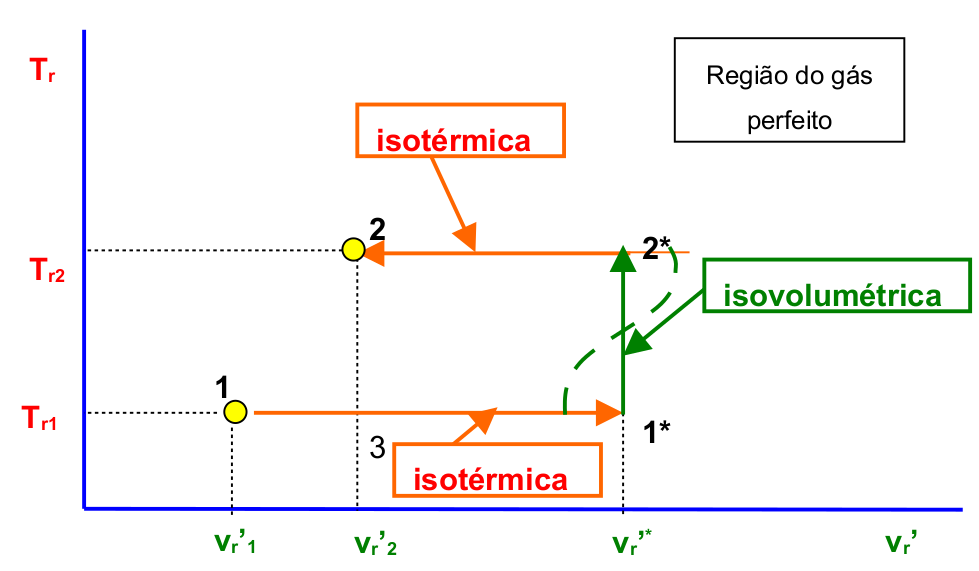
\includegraphics[%
            width=0.75\textwidth
        ]   {integrationPathThroughIdealGas.png}

        \label{fig:integrationPathThroughIdealGas}
    \end{figure}

    % Conferir com Prof. Woiski: os termos nos estados  1 e 2 estão trocados no
    % original, não?
    \begin{equation}
        \begin{aligned}
        \state{\gls{intInternalEnergy}}{2}
        \functionOf{
            \state{\gls{temperature}}{2},
            \state{\gls{specificVolume}}{2}
        }
        -
        \state{\gls{intInternalEnergy}}{1}
        \functionOf{
            \state{\gls{temperature}}{1},
            \state{\gls{specificVolume}}{1}
        }
        =&
        \state{
            \left(
                \idealgasprop{intInternalEnergy}
                -
                \gls{intInternalEnergy}
            \right)
        }{1}
        \functionOf{
            \state{\gls{temperature}}{1},
            \state{\gls{specificVolume}}{1}
        }
        -
        \state{
            \left(
                \idealgasprop{intInternalEnergy}
                -
                \gls{intInternalEnergy}
            \right)
        }{2}
        \functionOf{
            \state{\gls{temperature}}{2},
            \state{\gls{specificVolume}}{2}
        }\\
        &+
        \state{{\idealgasprop{intInternalEnergy}}}{2}
        \functionOf{
            \state{\gls{temperature}}{2}
        }
        -
        \state{{\idealgasprop{intInternalEnergy}}}{1}
        \functionOf{
            \state{\gls{temperature}}{1}
        }\,,
        \end{aligned}
    \end{equation}
    %
    onde
    %
    \begin{equation} \label{eq:6.6}
        \frac{
            \idealgasprop{intInternalEnergy}
            -
            \gls{intInternalEnergy}
        }{
            \gls{gasConstant}
            \gsub{temperature}{critical}
        }
        \functionOf{
            \gsub{temperature}{reduced},
            \gsub{specificVolume}{reduced}
        }
        =
        \int\limits_{\gls{modifiedReducedVolume}}^{\infty}{
            \frac{
                \gsub{temperature}{reduced}^2
            }{
                \gls{modifiedReducedVolume}
            }
            \ddxconsty{
                \gls{compressibilityFactor}
            }{
                \gsub{temperature}{reduced}
            }{
                \gls{modifiedReducedVolume}
            }
        }\diff{
            \gls{modifiedReducedVolume}
        }\,,
    \end{equation}
    %
    são as isotermas adimensionais até a região de gás perfeito. Observe que
    $\idealgasprop{intInternalEnergy} - \gls{intInternalEnergy}$ é definida
    como \emph{energia interna residual} ou \emph{desvio de energia interna do estado
    correspondente a \gls{intInternalEnergy}}, pois só é diferente de zero se
    no estado correspondente a \gls{intInternalEnergy} a substância não for gás
    perfeito. Esta é a mesma razão pela qual o limite superior de integração
    pode ser infinito. Ainda,
    %
    \begin{equation} \label{eq:6.7}
        \state{{\idealgasprop{intInternalEnergy}}}{2}
        \functionOf{
            \state{\gls{temperature}}{2}
        }
        -
        \state{{\idealgasprop{intInternalEnergy}}}{1}
        \functionOf{
            \state{\gls{temperature}}{1}
        }
        =
        \int\limits_{
            \state{\gls{temperature}}{1}
        }^{
            \state{\gls{temperature}}{2}
            }{
            \idealgasprop{constVolumeSpecificHeat}
            \functionOf{
                \gls{temperature}
            }
        }\diff{\gls{temperature}}\,,
    \end{equation}
    %
    é a integral de
    \idealgasprop{constVolumeSpecificHeat}\functionOf{\gls{temperature}} entre
    \state{\gls{temperature}}{1} e \state{\gls{temperature}}{2} na região do
    gás perfeito, cujo caminho de integração não precisa nem sequer ser
    isovolumétrico (por quê?).


    \section{A Entalpia em Coordenadas Generalizadas}

    Para a avaliação da entalpia, temos:
    %
    \begin{equation} \label{eq:6.8}
    \begin{aligned}
        \state{\gls{intEnthalpy}}{2}
        \functionOf{
            \state{\gls{temperature}}{2},
            \state{\gls{pressure}}{2}
        }
        -
        \state{\gls{intEnthalpy}}{1}
        \functionOf{
            \state{\gls{temperature}}{1},
            \state{\gls{pressure}}{1}
        }
        =&%
        \state{\gls{intInternalEnergy}}{2}
        \functionOf{
            \state{\gls{temperature}}{2},
            \state{\gls{pressure}}{2}
        }
        -
        \state{\gls{intInternalEnergy}}{1}
        \functionOf{
            \state{\gls{temperature}}{1},
            \state{\gls{pressure}}{1}
        }\\
        &+
        \state{\gls{pressure}}{2}
        \state{\gls{specificVolume}}{2}
        \functionOf{
            \state{\gls{temperature}}{2},
            \state{\gls{pressure}}{2}
        }
        -
        \state{\gls{pressure}}{1}
        \state{\gls{specificVolume}}{1}
        \functionOf{
            \state{\gls{temperature}}{1},
            \state{\gls{pressure}}{1}
        }\,.
    \end{aligned}
    \end{equation}

    Portanto, podemos facilmente mostrar que (faça-o como exercício!)
    %
    \begin{equation} \label{eq:6.9}
        \frac{
            \idealgasprop{intEnthalpy}
            -
            \gls{intEnthalpy}
        }{
            \gls{gasConstant}
            \gsub{temperature}{critical}
        }
        \functionOf{
            \gsub{temperature}{reduced},
            \gsub{specificVolume}{reduced},
            \gls{PitzerAcentricFactor},
            \gls{WuPolarFactor}
        }
        =
        \frac{
            \idealgasprop{intInternalEnergy}
            -
            \gls{intInternalEnergy}
        }{
            \gls{gasConstant}
            \gsub{temperature}{critical}
        }
        \functionOf{
            \gsub{temperature}{reduced},
            \gsub{specificVolume}{reduced},
            \gls{PitzerAcentricFactor},
            \gls{WuPolarFactor}
        }
        +
        \gsub{temperature}{reduced}
        \left[
            1
            -
            \gls{compressibilityFactor}
            \functionOf{
                \gsub{temperature}{reduced},
                \gsub{specificVolume}{reduced},
                \gls{PitzerAcentricFactor},
                \gls{WuPolarFactor}
            }
        \right]\,.
    \end{equation}

    Utilizando a \cref{eq:5.42}, podemos demonstrar que (faça!)
    %
    \begin{equation} \label{eq:6.10}
        \frac{
            \idealgasprop{intEnthalpy}
            -
            \gls{intEnthalpy}
        }{
            \gls{gasConstant}
            \gsub{temperature}{critical}
        }
        \functionOf{
            \gsub{temperature}{reduced},
            \gsub{pressure}{reduced},
            \gls{PitzerAcentricFactor},
            \gls{WuPolarFactor}
        }
        =
        \int\limits_{0}^{\gsub{pressure}{reduced}}{
            \frac{
                \gsub{temperature}{reduced}^2
            }{
                \gsub{pressure}{reduced}
            }
            \ddxconsty{
                \gls{compressibilityFactor}
            }{
                \gsub{temperature}{reduced}
            }{
                \gsub{pressure}{reduced}
            }
            \functionOf{
                \gsub{temperature}{reduced},
                \gsub{pressure}{reduced},
                \gls{PitzerAcentricFactor},
                \gls{WuPolarFactor}
            }
        }\diff{
            \gsub{pressure}{reduced},
        }\,.
    \end{equation}

    Então, o desvio de entalpia (ou entalpia residual) pode ser obtido
    diretamente da energia interna residual (ou vice-versa) sem maiores
    dificuldades.

    Para completar, portanto, o cálculo da variação da entalpia entre dois
    estados 1 e 2, resta-nos apenas acrescentar a integração de
    \idealgasprop{constPressureSpecificHeat}\functionOf{\gls{temperature}},
    exatamente como o fizemos para a energia interna. O resultado torna-se:
    %
    \begin{equation} \label{eq:6.11}
        \begin{aligned}
        \state{\gls{intEnthalpy}}{2}
        \functionOf{
            \state{\gls{temperature}}{2},
            \state{\gls{pressure}}{2}
        }
        -\state{\gls{intEnthalpy}}{1}
        \functionOf{
            \state{\gls{temperature}}{1},
            \state{\gls{pressure}}{1}
        }
        =&
        \left[
            \state{
                \frac{
                    \idealgasprop{intEnthalpy}
                    -
                    \gls{intEnthalpy}
                }{
                    \gls{gasConstant}
                    \gsub{temperature}{critical}
                }
            }{1}
            \functionOf{
                \state{\gsub{temperature}{reduced}}{1},
                \state{\gsub{pressure}{reduced}}{1},
                \gls{PitzerAcentricFactor},
                \gls{WuPolarFactor}
            }
        \right]
        \gls{gasConstant}
        \gsub{temperature}{critical}\\
        &-
        \left[
            \state{
                \frac{
                    \idealgasprop{intEnthalpy}
                    -
                    \gls{intEnthalpy}
                }{
                    \gls{gasConstant}
                    \gsub{temperature}{critical}
                }
            }{2}
            \functionOf{
                \state{\gsub{temperature}{reduced}}{2},
                \state{\gsub{pressure}{reduced}}{2},
                \gls{PitzerAcentricFactor},
                \gls{WuPolarFactor}
            }
        \right]
        \gls{gasConstant}
        \gsub{temperature}{critical}\\
        &+
        \state{{\idealgasprop{intEnthalpy}}}{2}
        \functionOf{
            \state{\gls{temperature}}{2}
        }
        -
        \state{{\idealgasprop{intEnthalpy}}}{1}
        \functionOf{
            \state{\gls{temperature}}{1}
        }\,,
        \end{aligned}
    \end{equation}
    %
    onde
    %
    \begin{equation}
        \state{{\idealgasprop{intEnthalpy}}}{2}
        \functionOf{
            \state{\gls{temperature}}{2}
        }
        -
        \state{{\idealgasprop{intEnthalpy}}}{1}
        \functionOf{
            \state{\gls{temperature}}{1}
        }
        =
        \int\limits_{
            \state{\gls{temperature}}{1}
        }^{
            \state{\gls{temperature}}{2}
        }{
            \idealgasprop{constPressureSpecificHeat}
            \functionOf{
                \gls{temperature}
            }
        }\diff{\gls{temperature}}\,.
    \end{equation}


    \section{A Entropia em Coordenadas Generalizadas}

    Infelizmente o esquema exposto não dará certo para a entropia, pois esta
    depende de \gls{specificVolume} ou de \gls{pressure} mesmo na região do gás
    perfeito. A isotérmica da entropia em coordenadas generalizadas é dada por:
    %
    \begin{equation} \label{eq:6.12}
        \frac{
            \idealgasprop{intEntropy}_{\idealgasprop{modifiedReducedVolume}}
            \functionOf{
                \gsub{temperature}{reduced},
                \idealgasprop{modifiedReducedVolume}
            }
            -
            \gls{intEntropy}_{\gls{modifiedReducedVolume}}
            \functionOf{
                \gsub{temperature}{reduced},
                \gls{modifiedReducedVolume}
            }
        }{
            \gls{gasConstant}
        }
        =
        \int\limits_{
            \gls{modifiedReducedVolume}
        }^{
            \idealgasprop{modifiedReducedVolume}
        }{
            \frac{1}{\gls{modifiedReducedVolume}}
            \left[
                \gls{compressibilityFactor}
                \functionOf{
                    \gsub{temperature}{reduced},
                    \gls{modifiedReducedVolume}
                }
                +
                \gsub{temperature}{reduced}
                \ddxconsty{
                    \gls{compressibilityFactor}
                }{
                    \gsub{temperature}{reduced}
                }{
                    \gls{modifiedReducedVolume}
                }
            \right]
        }\diff{
            \gls{modifiedReducedVolume}
        }\,.
    \end{equation}
    %
    e %
    $
        \lim\limits_{
            \idealgasprop{modifiedReducedVolume} \rightarrow \infty
        }{
            \int\limits_{
                \gls{modifiedReducedVolume}
            }^{
                \idealgasprop{modifiedReducedVolume}
            }{
                \frac{
                    \diff{\gls{modifiedReducedVolume}}
                }{
                    \gls{modifiedReducedVolume}
                }
            }
        } = \infty
    $, donde concluímos que a integral se torna ilimitada, o que não nos
    interessa nem um pouco. Façamos então:

    \begin{equation} \label{eq:6.13}
        \frac{
            \idealgasprop{intEntropy}_{\idealgasprop{modifiedReducedVolume}}
            \functionOf{
                \gsub{temperature}{reduced},
                \idealgasprop{modifiedReducedVolume}
            }
            -
            \idealgasprop{intEntropy}_{\gls{modifiedReducedVolume}}
            \functionOf{
                \gsub{temperature}{reduced},
                \gls{modifiedReducedVolume}
            }
        }{
            \gls{gasConstant}
        }
        =
        \ln{
            \left(
                \frac{
                    \idealgasprop{modifiedReducedVolume}
                }{
                    \gls{modifiedReducedVolume}
                }
            \right)
        }
        =
        \int\limits_{
            \gls{modifiedReducedVolume}
        }^{
            \idealgasprop{modifiedReducedVolume}
        }{
            \frac{
                1
            }{
                \gls{modifiedReducedVolume}
            }
        }\diff{\gls{modifiedReducedVolume}}\,,
    \end{equation}
    %
    onde $\idealgasprop{intEntropy}_{\gls{modifiedReducedVolume}}$ é o valor que
    a entropia teria, se assumíssemos gás perfeito em
    \gls{temperature},\gls{modifiedReducedVolume}, ou seja, um estado de gás
    perfeito hipotético.  Resta-nos, então, cancelarmos as singularidades,
    subtraindo a \cref{eq:6.13} da \cref{eq:6.12} (mostre!):
    %
    \begin{equation} \label{eq:6.14}
        \frac{
            \idealgasprop{intEntropy}
            -
            \gls{intEntropy}
        }{
            \gls{gasConstant}
        }
        \functionOf{
            \gsub{temperature}{reduced},
            \gls{modifiedReducedVolume}
        }
        =
        \int\limits_{
            \gls{modifiedReducedVolume}
        }^{
            \infty
        }{
            \frac{1}{\gls{modifiedReducedVolume}}
            \left[
                \gls{compressibilityFactor}
                \functionOf{
                    \gsub{temperature}{reduced},
                    \gls{modifiedReducedVolume}
                }
                +
                \gsub{temperature}{reduced}
                \ddxconsty{
                    \gls{compressibilityFactor}
                }{
                    \gsub{temperature}{reduced}
                }{
                    \gls{modifiedReducedVolume}
                }
                \functionOf{
                    \gsub{temperature}{reduced},
                    \gls{modifiedReducedVolume}
                }
                -
                1
            \right]
        }\diff{
            \gls{modifiedReducedVolume}
        }\,.
    \end{equation}

    Assim, o desvio de entropia (ou entropia residual) é calculado no estado
    \gsub{temperature}{reduced},\gls{modifiedReducedVolume} em relação ao valor
    que a entropia teria se fosse gás perfeito hipotético neste mesmo estado.

    Observe que os estados hipotéticos não serão incomuns em nosso estudo. Isso
    não deve nos assustar, pois sempre estarão acompanhados das devidas
    correções que darão conta dos desvios entre a hipótese e o estado físico
    real. De fato, os nossos primeiros exemplos dessas correções são exatamente
    os desvios de energia interna, entalpia e de entropia.

    Raciocinando de forma análoga, obtemos o desvio de entropia adimensional em
    função de \gsub{temperature}{reduced}, \gsub{pressure}{reduced},
    \gls{PitzerAcentricFactor}, \gls{WuPolarFactor} (faça!):
    %
    \begin{equation} \label{eq:6.15}
        \frac{
            \idealgasprop{intEntropy}
            -
            \gls{intEntropy}
        }{
            \gls{gasConstant}
        }
        \functionOf{
            \gsub{temperature}{reduced},
            \gsub{pressure}{reduced},
            \gls{PitzerAcentricFactor},
            \gls{WuPolarFactor}
        }
        =
        \int\limits_{
            0
        }^{
            \gsub{pressure}{reduced}
        }{
            \frac{1}{\gsub{pressure}{reduced}}
            \left[
                \gls{compressibilityFactor}
                \functionOf{
                    \gsub{temperature}{reduced},
                    \gsub{pressure}{reduced},
                    \gls{PitzerAcentricFactor},
                    \gls{WuPolarFactor}
                }
                +
                \gsub{temperature}{reduced}
                \ddxconsty{
                    \gls{compressibilityFactor}
                }{
                    \gsub{temperature}{reduced}
                }{
                    \gls{modifiedReducedVolume}
                }
                \functionOf{
                    \gsub{temperature}{reduced},
                    \gsub{pressure}{reduced},
                    \gls{PitzerAcentricFactor},
                    \gls{WuPolarFactor}
                }
                -
                1
            \right]
        }\diff{
            \gsub{pressure}{reduced}
        }\,.
    \end{equation}

    A diferença de entropia entre dois estados 1 e 2 será dada por:

    \begin{equation} \label{eq:6.16}
        \begin{aligned}
        \state{\gls{intEntropy}}{2}
        \functionOf{
            \state{\gls{temperature}}{2},
            \state{\gls{pressure}}{2}
        }
        -
        \state{\gls{intEntropy}}{1}
        \functionOf{
            \state{\gls{temperature}}{1},
            \state{\gls{pressure}}{1}
        }
        =&
        \left[
            \state{
                \frac{
                    \idealgasprop{intEntropy}
                    -
                    \gls{intEntropy}
                }{
                    \gls{gasConstant}
                }
            }{1}
            \functionOf{
                \state{\gsub{temperature}{reduced}}{1},
                \state{\gsub{pressure}{reduced}}{1},
                \gls{PitzerAcentricFactor},
                \gls{WuPolarFactor}
            }
        \right]
        \gls{gasConstant}\\
        &-
        \left[
            \state{
                \frac{
                    \idealgasprop{intEntropy}
                    -
                    \gls{intEntropy}
                }{
                    \gls{gasConstant}
                }
            }{2}
            \functionOf{
                \state{\gsub{temperature}{reduced}}{2},
                \state{\gsub{pressure}{reduced}}{2},
                \gls{PitzerAcentricFactor},
                \gls{WuPolarFactor}
            }
        \right]
        \gls{gasConstant}\\
        &+
        \state{{\idealgasprop{intEntropy}}}{2}
        \functionOf{
            \state{\gls{temperature}}{2},
            \state{\gls{pressure}}{2}
        }
        -
        \state{{\idealgasprop{intEntropy}}}{1}
        \functionOf{
            \state{\gls{temperature}}{1},
            \state{\gls{pressure}}{1}
        }\,,
        \end{aligned}
    \end{equation}
    %
    onde:
    %
    \begin{equation} \label{eq:6.17}
        \state{{\idealgasprop{intEntropy}}}{2}
        \functionOf{
            \state{\gls{temperature}}{2},
            \state{\gls{pressure}}{2}
        }
        -
        \state{{\idealgasprop{intEntropy}}}{1}
        \functionOf{
            \state{\gls{temperature}}{1},
            \state{\gls{pressure}}{1}
        }
        =
        \int\limits_{
            \state{\gls{temperature}}{1}
        }^{
            \state{\gls{temperature}}{2}
        }{
            \frac{
                \idealgasprop{constPressureSpecificHeat}
                \functionOf{
                    \gls{temperature}
                }
            }{
                \gls{temperature}
            }
        }\diff{\gls{temperature}}
        -
        \gls{gasConstant}
        \ln{
        \left(
            \frac{
                \state{\gls{pressure}}{2}
            }{
                \state{\gls{pressure}}{1}
            }
        \right)}\,.
    \end{equation}
    %
    ou então,
    %
    \begin{equation} \label{eq:6.18}
        \state{{\idealgasprop{intEntropy}}}{2}
        \functionOf{
            \state{\gls{temperature}}{2},
            \state{\gls{pressure}}{2}
        }
        -
        \state{{\idealgasprop{intEntropy}}}{1}
        \functionOf{
            \state{\gls{temperature}}{1},
            \state{\gls{pressure}}{1}
        }
        =
        \int\limits_{
            \state{\gls{temperature}}{1}
        }^{
            \state{\gls{temperature}}{2}
        }{
            \frac{
                \idealgasprop{constVolumeSpecificHeat}
                \functionOf{
                    \gls{temperature}
                }
            }{
                \gls{temperature}
            }
        }\diff{\gls{temperature}}
        +
        \gls{gasConstant}
        \ln{
        \left(
            \frac{
                \state{\gls{specificVolume}}{2}
            }{
                \state{\gls{specificVolume}}{1}
            }
        \right)}\,.
    \end{equation}

    Sabemos agora, em princípio, como expressar as diferenças de energia
    interna, \cref{eq:6.6}, de entalpia, \cref{eq:6.11}, bem como de entropia,
    \cref{eq:6.16}, para uma substância pura entre dois estados 1 e 2 em termos
    de diferenças relativas ao gás perfeito de energia interna, \cref{eq:6.7},
    entalpia, \cref{eq:6.12}, e entropia, \cref{eq:6.17,eq:6.18}, entre estes
    mesmos estados, devidamente alteradas pelos desvios de energia interna (ou
    energia interna residual), \cref{eq:6.6}, entalpia (ou entalpia residual),
    \cref{eq:6.10}, e entropia (ou entropia residual), \cref{eq:6.14}, ou
    \cref{eq:6.15}, em cada um destes estados.

    Sabemos como determinar numérica ou algebricamente as diferenças de energia
    interna, entalpia e entropia do gás perfeito entre dois estados, conhecendo
    uma expressão para os calores específicos de uma substância pura em função
    da temperatura \gls{temperature}.

    Resta-nos então determinar numericamente as energias internas, entalpias e
    entropias residuais em um dado estado. De maneira geral, devido a natureza
    complexa das equações de estado que serão utilizadas, as diferenciações e
    integrações nas equações terão que ser resolvidas de forma numérica,
    mediante programas de computador. Entretanto, antes de nos dedicarmos a
    esta tarefa, vamos definir uma propriedade termodinâmica bastante útil, a
    fugacidade.


    \section{A Fugacidade de Substâncias Puras}
    \label{sec:fugacityDefintion}

    Seja uma substância pura. Podemos escrever a parte isotérmica da relação
    fundamental na forma de função de Gibbs (molar) e substituir
    \molar{\gls{specificVolume}}:

    \begin{equation} \label{eq:6.19}
        \diff{
            \molar{\gls{intGibbsFreeEnergy}}
        }_{\gls{temperature}}
        =
        \molar{\gls{specificVolume}}
        \diff{\gls{pressure}}_{\gls{temperature}}
        =
        \frac{
            \gls{compressibilityFactor}
            \functionOf{
                \gls{pressure},
                \gls{temperature}
            }
            \gls{universalGasConstant}
            \gls{temperature}
        }{
            \gls{pressure}
        }
        \diff{\gls{pressure}}_{\gls{temperature}}
        =
        \gls{compressibilityFactor}
        \functionOf{
            \gls{pressure},
            \gls{temperature}
        }
        \gls{universalGasConstant}
        \gls{temperature}
        \diff{
            \left(
                \ln{\gls{pressure}}
            \right)
        }_{\gls{temperature}}\,.
    \end{equation}

    Por outro lado, para o gás perfeito, temos:

    \begin{equation} \label{eq:6.20}
        \diff{
            \molar{\gls{intGibbsFreeEnergy}}
        }_{\gls{temperature}}
        =
        \molalidealgasprop{specificVolume}
        \diff{\gls{pressure}}_{\gls{temperature}}
        =
        \frac{
            \gls{universalGasConstant}
            \gls{temperature}
        }{
            \gls{pressure}
        }
        \diff{\gls{pressure}}_{\gls{temperature}}
        =
        \gls{universalGasConstant}
        \gls{temperature}
        \diff{
            \left(
                \ln{\gls{pressure}}
            \right)
        }_{\gls{temperature}}\,.
    \end{equation}

    Comparando as duas expressões, percebemos que em vez de colocarmos sobre
    \gls{compressibilityFactor} o fato de ser ou não gás perfeito, podemos
    definir uma nova propriedade termodinâmica que chamaremos de fugacidade
    \gls{fugacity} da seguinte forma:
    %
    \begin{equation} \label{eq:6.21}
        \diff{
            \molar{\gls{intGibbsFreeEnergy}}
        }_{\gls{temperature}}
        =
        \molar{\gls{specificVolume}}
        \functionOf{
            \gls{pressure},
            \gls{temperature}
        }
        \diff{\gls{pressure}}_{\gls{temperature}}
        =
        \frac{
            \gls{compressibilityFactor}
            \functionOf{
                \gls{pressure},
                \gls{temperature}
            }
            \gls{universalGasConstant}
            \gls{temperature}
        }{
            \gls{pressure}
        }
        \diff{\gls{pressure}}_{\gls{temperature}}
        =
        \gls{universalGasConstant}
        \gls{temperature}
        \diff{
            \left[
                \ln{
                    \gls{fugacity}
                    \functionOf{
                        \gls{pressure},
                        \gls{temperature}
                    }
                }
            \right]
        }_{\gls{temperature}}\,,
    \end{equation}
    %
    desde que
    %
    \begin{equation}
        \lim\limits_{\gls{pressure} \rightarrow 0}{
            \left(
                \frac{
                    \gls{fugacity}
                }{
                    \gls{pressure}
                }
                \functionOf{
                    \gls{pressure},
                    \gls{temperature}
                }
            \right)
        }
        =
        1\,.
    \end{equation}

    Em outras palavras, em vez de usarmos \gls{compressibilityFactor} para
    enfatizarmos a diferença de não ser gás perfeito, podemos criar efeito
    semelhante, quando substituirmos \gls{fugacity} no lugar de \gls{pressure}
    nas equações. Por essa razão, a fugacidade é chamada também de
    \emph{pseudo-pressão}. Você pode facilmente mostrar que na região do gás
    perfeito a fugacidade coincide com a pressão (faça!).

    A fugacidade, como qualquer outra propriedade termodinâmica intensiva, é
    uma função de duas propriedades intensivas independentes e, portanto,
    também pode ser expressa em coordenadas generalizadas, da seguinte forma
    (você deve mostrar isso, integrando e adimensionalizando a
    \cref{eq:6.20}...):
    %
    \begin{equation} \label{eq:6.22}
        \ln{
            \left(
                \frac{
                    \gls{fugacity}
                }{
                    \gls{pressure}
                }
            \right)_{\gsub{temperature}{reduced}}
        }
        \functionOf{
            \gsub{temperature}{reduced},
            \gsub{pressure}{reduced},
            \gls{PitzerAcentricFactor},
            \gls{WuPolarFactor}
        }
        =
        \int\limits_{0}^{\gsub{pressure}{reduced}}{
            \left[
                \gls{compressibilityFactor}
                \functionOf{
                    \gsub{temperature}{reduced},
                    \gsub{pressure}{reduced},
                    \gls{PitzerAcentricFactor},
                    \gls{WuPolarFactor}
                }
                -
                1
            \right]
        }\diff{
            \left(
                \ln{\gsub{pressure}{reduced}}
            \right)
        }_{\gsub{temperature}{reduced}}\,,
    \end{equation}
    %
    onde o adimensional $\frac{\gls{fugacity}}{\gls{pressure}}$, ou o seu
    logaritmo, é denominado \emph{coeficiente de fugacidade}.

    Com o que aprendeu até agora, você deve ser capaz de demonstrar a
    identidade adimensional:
    %
    \begin{equation}
    \begin{aligned}
        \ln{
            \left(
                \frac{
                    \gls{fugacity}
                }{
                    \gls{pressure}
                }
            \right)_{\gsub{temperature}{reduced}}
        }
        \functionOf{
            \gsub{temperature}{reduced},
            \gsub{pressure}{reduced},
            \gls{PitzerAcentricFactor},
            \gls{WuPolarFactor}
        }
        &=
        -
        \frac{1}{\gsub{temperature}{reduced}}
        \left(
            \frac{
                \idealgasprop{intGibbsFreeEnergy}
                -
                \gls{intGibbsFreeEnergy}
            }{
                \gls{gasConstant}
                \gsub{temperature}{critical}
            }
        \right)
        \functionOf{
            \gsub{temperature}{reduced},
            \gsub{pressure}{reduced},
            \gls{PitzerAcentricFactor},
            \gls{WuPolarFactor}
        }\\
        &=
        -
        \frac{1}{\gsub{temperature}{reduced}}
        \left(
            \frac{
                \idealgasprop{intEnthalpy}
                -
                \gls{intEnthalpy}
            }{
                \gls{gasConstant}
                \gsub{temperature}{critical}
            }
        \right)
        \functionOf{
            \gsub{temperature}{reduced},
            \gsub{pressure}{reduced},
            \gls{PitzerAcentricFactor},
            \gls{WuPolarFactor}
        }
        +
        \left(
            \frac{
                \idealgasprop{intEntropy}
                -
                \gls{intEntropy}
            }{
                \gls{gasConstant}
            }
        \right)
        \functionOf{
            \gsub{temperature}{reduced},
            \gsub{pressure}{reduced},
            \gls{PitzerAcentricFactor},
            \gls{WuPolarFactor}
        }\,.
    \end{aligned}
    \end{equation}


    \section{%
        Os Diagramas Generalizados com Lee-Kesler e Fluidos Simples
    }

    Se admitirmos a validade universal da Regra dos Estados Correspondentes,
    então, de posse de uma --- ou de mais de uma --- equação de estado
    confiável expressa na forma generalizada, tal como a equação de estado de
    Lee-Kesler, podemos, com ajuda do computador, proceder às necessárias
    derivações e integrações numéricas e tabular os dados resultantes.
    Historicamente, têm sido comuns as tabelas contendo o fator de
    compressibilidade, o desvio de entalpia e o desvio de entropia, como função
    das variáveis \gsub{pressure}{reduced} e \gsub{temperature}{reduced}, não
    apenas para a região de vapor superaquecido, mas também para as regiões de
    saturação e de líquido comprimido.

    De posse das tabelas ou programas de computador, se você souber o que está
    fazendo, não precisa nem se preocupar com o desenvolvimento matemático
    anterior.

    Vejamos um exemplo: \emph{Estrangula-se metano de \SI{2}{\mega\pascal} e
    \SI{25}{\celsius} a \SI{0.1}{\mega\pascal} num processo adiabático e em
    regime permanente. Determine a temperatura final do metano.}

    Pela Primeira Lei, desprezando-se as energias cinética e potencial, como
    não existe trabalho e nem calor:
    %
    \begin{equation}
        \gsub{intEnthalpy}{inlet}
        =
        \gsub{intEnthalpy}{outlet}\,,
    \end{equation}
    %
    onde $\gsub{intEnthalpy}{inlet} =
    \gls{intEnthalpy}\functionOf{\gsub{pressure}{inlet},
    \gsub{temperature}{inlet}}$ e $\gsub{intEnthalpy}{outlet} =
    \gls{intEnthalpy}\functionOf{\gsub{pressure}{outlet},
    \gsub{temperature}{outlet}}$, com \gsub{temperature}{outlet} desconhecido.
    Para podermos utilizar coordenadas generalizadas precisamos obter
    \gsub{pressure}{critical}, \gsub{temperature}{critical}, \gls{gasConstant}
    e \idealgasprop{constPressureSpecificHeat} do metano:
    %
    \begin{equation*}
    \begin{aligned}
        \gsub{pressure}{critical} &= \SI{4.60}{\mega\pascal}\,,\\
        \gsub{temperature}{critical} &= \SI{190.4}{\kelvin}\,,\\
        \gls{gasConstant}
        &=
        \SI{0.51832}{\kilo\joule\per\kilo\gram\per\kelvin}\,,\\
        \idealgasprop{constPressureSpecificHeat}
        &=
        \SI{2.2537}{\kilo\joule\per\kilo\gram\per\kelvin}\,.
    \end{aligned}
    \end{equation*}
    %
    e, então, determinar \gsub{temperature}{reduced} e
    \gsub{pressure}{reduced}:
    %
    \begin{equation*}
    \begin{aligned}
        \gsub{temperature}{reduced,inlet}
        &=
        \frac{\num{298.15}}{\num{190.4}}
        =
        \num{1.566}\,,\\
        %
        \gsub{pressure}{reduced,inlet}
        &=
        \frac{\num{2.0}}{\num{4.60}}
        =
        \num{0.4347}\,,\\
        %
        \gsub{pressure}{reduced,outlet}
        &=
        \frac{\num{0.1}}{\num{4.60}}
        =
        \num{0.0217}\,.\\
    \end{aligned}
    \end{equation*}

    Por outro lado, expandindo-se a entalpia:
    %
    \begin{equation} \label{eq:6.23}
        \gsub{intEnthalpy}{inlet}
        -
        \gsub{intEnthalpy}{outlet}
        =
        \left(
            \idealgasprop{intEnthalpy}_{\gls{outlet}}
            -
            \gsub{intEnthalpy}{outlet}
        \right)
        \functionOf{
            \gsub{temperature}{reduced,outlet},
            \gsub{pressure}{reduced,outlet}
        }
        -
        \left(
            \idealgasprop{intEnthalpy}_{\gls{inlet}}
            -
            \gsub{intEnthalpy}{inlet}
        \right)
        \functionOf{
            \gsub{temperature}{reduced,inlet},
            \gsub{pressure}{reduced,inlet}
        }
        +
        \left[
            \idealgasprop{intEnthalpy}_{\gls{inlet}}
            \functionOf{
                \gsub{temperature}{inlet}
            }
            -
            \idealgasprop{intEnthalpy}_{\gls{outlet}}
            \functionOf{
                \gsub{temperature}{outlet}
            }
        \right]
        =
        0\,,
    \end{equation}

    na qual o primeiro termo depende de \gsub{temperature}{reduced,outlet},
    \gsub{pressure}{reduced,outlet}, o termo intermediário depende de
    \gsub{temperature}{reduced,inlet}, \gsub{pressure}{reduced,inlet} e o
    último termo representa a integral do calor específico de
    \gsub{temperature}{inlet} até \gsub{temperature}{outlet}. Observe que,
    embora a única incógnita seja \gsub{temperature}{outlet} (ou
    \gsub{temperature}{reduced,outlet}), a solução deve ser encontrada por
    iteração.

    Vamos então encontrar a solução, admitindo que o estado de saída não é
    saturado, mas que o calor específico do gás perfeito não pode ser
    considerado constante.

    Das tabelas de entalpia residual com $\gls{PitzerAcentricFactor} = 0$, para
    $\gsub{temperature}{reduced,inlet} = \num{1.566}$ e
    $\gsub{pressure}{reduced,inlet} = \num{0.4347}$, %
    $
        \idealgasprop{intEnthalpy}_{\gls{inlet}}
        -
        \gsub{intEnthalpy}{inlet}
        =
        \num{0.19581} \times \num{0.51835} \times \num{190.4}
        =
        \SI{19.325}{\kilo\joule\per\kilo\gram\per\kelvin}
    $ e a equação final se torna:
    %
    \begin{equation} \label{eq:6.24}
        \begin{aligned}
        \idealgasprop{intEnthalpy}_{\gls{inlet}}
        \functionOf{
            \SI{298.15}{\kelvin}
        }
        -
        \idealgasprop{intEnthalpy}_{\gls{outlet}}
        \functionOf{
            \gsub{temperature}{outlet}
        }
        &+
        \left[
            \left(
                \frac{
                    \idealgasprop{intEnthalpy}_{\gls{outlet}}
                    -
                    \gsub{intEnthalpy}{outlet}
                }{
                    \gls{gasConstant}
                    \gsub{temperature}{critical}
                }
            \right)
            \functionOf{
                \gsub{temperature}{reduced,outlet},
                \frac{\num{2.0}}{\num{4.60}}
            }
        \right]
        \left(
            \SI[per-mode=fraction]{0.51832}{\kilo\joule\per\kilo\gram\per\kelvin}
        \right)
        \left(
            \SI{190.4}{\kelvin}
        \right)\\
        &-
        \left(
            \SI[per-mode=fraction]{19.325}{\kilo\joule\per\kilo\gram\per\kelvin}
        \right)
        =
        0\,,
        \end{aligned}
    \end{equation}

    A partir da formulação do problema, o sistema de equações se resume a uma
    equação e uma incógnita, mas infelizmente a solução é necessariamente
    iterativa. Como \gls{PitzerAcentricFactor} do \ch{CH4} é igual a
    \num{0.011}, poderíamos lançar mão das tabelas para obter por interpolação
    reversa a temperatura, mas ainda restaria a determinação da entalpia do gás
    perfeito, complicada pela hipótese de calor específico variável.

    Na próxima seção abordaremos os aspectos computacionais que nos habilitarão
    a resolver problemas muito mais complexos do que este.


    \section{%
        O Programa {LK\_WS\_NR} e o pacote {LK\_proptermo}
    }

    Utilizando a equação de estado de Lee-Kesler na forma generalizada, o fator
    acêntrico de Pitzer e o fator de correção de Wu-Stiel, desenvolvemos em
    Python o aplicativo denominado \command{LK\_proptermo}. Python é uma
    linguagem de programação de código aberto, muito alto nível, interpretada
    para uma máquina virtual, orientada a objetos, de tipagem dinâmica,
    multiplataforma e de sintaxe simples.

    Para podermos obter as propriedades termodinâmicas de uma substância pura,
    além de Python 3 e do pacote \command{LK\_proptermo}, são necessários
    ainda: a biblioteca NumPy, para a construção de arrays multidimensionais; o
    módulo \command{robustNR\_args}, para a obtenção de raízes de sistemas de
    equações não lineares por um método modificado de Newton-Raphson, com
    jacobiano sintético; a base de dados \command{tabelaA1A3.db}, contendo as
    propriedades das Tabelas A1 e A3 do livro do Assael e o módulo
    \command{a1\_assael}, para se obter  a assinatura da substância pura,
    \gls{molecularMass}, \gsub{temperature}{critical},
    \gsub{pressure}{critical}, \gls{PitzerAcentricFactor}, \gls{WuPolarFactor}
    além do calor específico, entalpia e entropia do gás perfeito em função da
    temperatura e pressão, dados por polinômios.

    Colocamos a seguir, para referência imediata, as docstrings dos módulos bem
    como as tabelas com os resultados calculados com os módulos e aqueles
    obtidos através das tabelas do Van Wylen, quarta edição, para os casos da
    amônia e da água. Note que os erros relativos para os estados selecionados
    são menores do que \SI{0.5}{\percent}.

    \begin{Verbatim}[baselinestretch=1.0]
                NH3 - VALORES CALCULADOS E TABELADOS
    (1) T1,P1 = -20+273.15,0.125 [K,MPa] (2) T2,P2 = 160+273.15,1.8  [K,MPa]
    ------------------------------------------------------------------------
           CALCULADO           TABELADO       UNIDADES     ERRO RELATIVO
           LK_WS_NR +          TAB. A.2.2                  AO VALOR TABELADO
           proptermo_assael    Van Wylen 4a                       (%)
    ------------------------------------------------------------------------
    v1     0.96590404593       0.9627         m3/kg        0.333
    v2     0.112416095135      0.1119         m3/kg        0.461
    h2-h1  370.272193283       368.6          kJ/kg        0.454
    u2-u1  288.661227781       287.5175       kJ/kg        0.398
    s2-s1 -0.161305216348     -0.1608         kJ/kgk       0.314
    ------------------------------------------------------------------------
    \end{Verbatim}


    \begin{Verbatim}[baselinestretch=1.0]
                 H2O -  VALORES CALCULADOS E TABELADOS
    (1) T1,P1 = 50+273.15,0.01 [K,MPa]   (2) T2,P2 = 200+273.15,10.  [K,MPa]
    -----------------------------------------------------------------------
           CALCULADO           TABELADO       UNIDADES    ERRO RELATIVO
           LK_WS_NR +          TAB. A.2.2                 AO VALOR TABELADO
           proptermo_assael    Van Wylen 4a                      (%)
    -----------------------------------------------------------------------
    v1     14.8700386541        14.869         m3/kg      0.007
    v      20.00114517466568    0.001148       m3/kg      0.246
    h2-h1 -1735.08696825       -1736.63        kJ/kg      0.089
    u2-u1 -1597.83832836       -1599.41        kJ/kg      0.098
    s2-s1 -5.85442128058       -5.8571         kJ/kgk     0.046
    -----------------------------------------------------------------------
    \end{Verbatim}

    \section{A Questão das Bases Arbitrárias}

    Você já aprendeu, com tudo o que desenvolvemos até agora, que o valor
    absoluto das propriedades termodinâmicas das substâncias puras não tem
    significado a não ser relativamente a uma base arbitrária. Por outro lado,
    para que as leis da termodinâmica tenham consistência física, a diferença
    das propriedades termodinâmicas entre dois estados tem que ser independente
    de qualquer base, ou seja, é invariante. Vamos utilizar este fato em nosso
    próprio benefício para simplificar consideravelmente a nossa interface
    computacional.

    Seja uma substância pura tal que escolhe-se um valor arbitrário para a
    entalpia \gsub{intEnthalpy}{base}\functionOf{\gsub{temperature}{base},
    \gsub{pressure}{base}} e um valor arbitrário para a entropia
    \gsub{intEntropy}{base}\functionOf{\gsub{temperature}{base},
    \gsub{pressure}{base}} em um mesmo estado de referência (base) \gls{base}.
    A rigor, nem precisariam ser o mesmo estado de referência para a entalpia e
    para a entropia, mas adotaremos o mesmo estado \gls{base} por simplicidade
    e a mesma hipótese foi implementada no \command{LK\_proptermo}. Aprendemos
    que podemos expressar, então, a entalpia
    \gls{intEnthalpy}\functionOf{\gls{temperature}, \gls{pressure}} e a
    entropia \gls{intEnthalpy}\functionOf{\gls{temperature}, \gls{pressure}} em
    um estado qualquer \gls{temperature}, \gls{pressure} em:
    %
    \begin{equation} \label{eq:6.25}
        \gls{intEnthalpy}
        \functionOf{
            \gls{temperature},
            \gls{pressure}
        }
        =
        \gsub{intEnthalpy}{base}
        +
        \left(
            \idealgasprop{intEnthalpy}
            -
            \gls{intEnthalpy}
        \right)_{\gls{base}}
        \functionOf{
            \gsub{temperature}{base},
            \gsub{pressure}{base}
        }
        -
        \left(
            \idealgasprop{intEnthalpy}
            -
            \gls{intEnthalpy}
        \right)
        \functionOf{
            \gls{temperature},
            \gls{pressure}
        }
        +
        \left[
            \idealgasprop{intEnthalpy}
            \functionOf{
                \gls{temperature}
            }
            -
            \idealgasprop{intEnthalpy}_{\gls{base}}
            \functionOf{
                \gsub{temperature}{base}
            }
        \right]\,,
    \end{equation}
    %
    e
    %
    \begin{equation} \label{eq:6.26}
        \gls{intEntropy}
        \functionOf{
            \gls{temperature},
            \gls{pressure}
        }
        =
        \gsub{intEntropy}{base}
        +
        \left(
            \idealgasprop{intEntropy}
            -
            \gls{intEntropy}
        \right)_{\gls{base}}
        \functionOf{
            \gsub{temperature}{base},
            \gsub{pressure}{base}
        }
        -
        \left(
            \idealgasprop{intEntropy}
            -
            \gls{intEntropy}
        \right)
        \functionOf{
            \gls{temperature},
            \gls{pressure}
        }
        +
        \left[
            \idealgasprop{intEntropy}
            \functionOf{
                \gls{temperature},
                \gls{pressure}
            }
            -
            \idealgasprop{intEntropy}_{\gls{base}}
            \functionOf{
                \gsub{temperature}{base},
                \gsub{pressure}{base}
            }
        \right]\,.
    \end{equation}

    Nestas expressões, aprenda de uma vez por todas a distinguir os
    desvios dimensionais %
    $
        \left(
            \idealgasprop{intEnthalpy}
            -
            \gls{intEnthalpy}
        \right)
        \functionOf{
            \gls{temperature},
            \gls{pressure}
        }
    $ (ou %
    $
        (
            \molalidealgasprop{intEnthalpy}
            -
            \molar{\gls{intEnthalpy}}
        )
        \functionOf{
            \gls{temperature},
            \gls{pressure}
        }
    $) e %
    $
        \left(
            \idealgasprop{intEntropy}
            -
            \gls{intEntropy}
        \right)
        \functionOf{
            \gls{temperature},
            \gls{pressure}
        }
    $ (ou %
    $
        \left(
            \molalidealgasprop{intEntropy}
            -
            \molar{\gls{intEntropy}}
        \right)
        \functionOf{
            \gls{temperature},
            \gls{pressure}
        }
    $) %
    das contrapartidas adimensionais: %
    $
        \left(
            \dfrac{
                \idealgasprop{intEnthalpy}
                -
                \gls{intEnthalpy}
            }{
                \gls{gasConstant}
                \gsub{temperature}{critical}
            }
        \right)
        \functionOf{
            \gsub{temperature}{reduced},
            \gsub{pressure}{reduced},
            \gls{PitzerAcentricFactor},
            \gls{WuPolarFactor}
        }
    $ e %
    $
        \left(
            \dfrac{
                \idealgasprop{intEntropy}
                -
                \gls{intEntropy}
            }{
                \gls{gasConstant}
                \gsub{temperature}{critical}
            }
        \right)
        \functionOf{
            \gsub{temperature}{reduced},
            \gsub{pressure}{reduced},
            \gls{PitzerAcentricFactor},
            \gls{WuPolarFactor}
        }
    $.

    As \cref{eq:6.25,eq:6.26} podem ser remanejadas da seguinte maneira:
    %
    \begin{equation} \label{eq:6.27}
        \gls{intEnthalpy}
        \functionOf{
            \gls{temperature},
            \gls{pressure}
        }
        =
        \left[
            \gsub{intEnthalpy}{base}
            +
            \left(
                \idealgasprop{intEnthalpy}
                -
                \gls{intEnthalpy}
            \right)_{\gls{base}}
            -
            \idealgasprop{intEnthalpy}_{\gls{base}}
        \right]
        \functionOf{
            \gsub{temperature}{base},
            \gsub{pressure}{base}
        }
        -
        \left(
            \idealgasprop{intEnthalpy}
            -
            \gls{intEnthalpy}
        \right)
        \functionOf{
            \gls{temperature},
            \gls{pressure}
        }
        +
        \idealgasprop{intEnthalpy}
        \functionOf{
            \gls{temperature}
        }\,,
    \end{equation}
    %
    e
    %
    \begin{equation} \label{eq:6.28}
        \gls{intEntropy}
        \functionOf{
            \gls{temperature},
            \gls{pressure}
        }
        =
        \left[
            \gsub{intEntropy}{base}
            +
            \left(
                \idealgasprop{intEntropy}
                -
                \gls{intEntropy}
            \right)_{\gls{base}}
            -
            \idealgasprop{intEntropy}_{\gls{base}}
        \right]
        \functionOf{
            \gsub{temperature}{base},
            \gsub{pressure}{base}
        }
        -
        \left(
            \idealgasprop{intEntropy}
            -
            \gls{intEntropy}
        \right)
        \functionOf{
            \gls{temperature},
            \gls{pressure}
        }
        +
        \idealgasprop{intEntropy}
        \functionOf{
            \gls{temperature},
            \gls{pressure}
        }\,.
    \end{equation}

    Observe que, \emph{uma vez que os termos entre colchetes já foram
    calculados quando da definição da base \gls{base}}, o estado fixado por
    $(\gls{temperature},\gls{pressure})$ será obtido apenas pela determinação
    das entalpias e das entropias residuais, bem como pelas propriedades do gás
    perfeito da substância pura em questão a
    $(\gls{temperature},\gls{pressure})$. Salientamos que o estado
    correspondente à base escolhida para uma determinada substância pura ou
    deve ser real (determinável) para aquela substância pura, ou então, sob
    determinadas circunstâncias, ser adotada como gás perfeito (real ou
    hipotético). Esta última escolha da base --- sob as circunstâncias certas
    --- nos será muito útil quando precisarmos definir e utilizar as bases
    termoquímicas para misturas reativas. A base pode ser um estado saturado a
    $(\gsub{temperature}{base},\gsub{vaporQuality}{base})$ ou
    $(\gsub{pressure}{base},\gsub{vaporQuality}{base})$. Além disso, o próprio
    estado a ser determinado pode ser saturado a
    $(\gls{temperature},\gls{vaporQuality})$ ou
    $(\gls{pressure},\gls{vaporQuality})$. Como ficariam as
    \cref{eq:6.27,eq:6.28}? E se o estado a ser determinado, ou a base, ou
    ambos, forem gases perfeitos (faça!)?


    \section{Um Exemplo com a Amônia}

    Veja a seguir um exemplo, executando-se o pacote \command{LK\_proptermo},
    com o refrigerante amônia, considerando-se uma base compatível com as
    tabelas termodinâmicas do livro do Van Wylen, para efeito de comparação:

    \begin{Verbatim}[baselinestretch=1.0,fontsize=\scriptsize]
    Tb,xb = -40.+273.15,0.
    T1,P1 = -50.+273.15,1.
    T2,P2 = 30. + 273.15, 0.1
    base = Base(Tb=Tb,xb=xb) # Usou-se a mesma base para todos os refrigerantes (VW)...

    A instância da classe State representa o estado real da substância pura
    <sub> a (T,P) ou (T,x) ou (P,x), fornecidos os valores de base, uma
    instância da classe Base cujo construtor são os valores para a base:
    hb,sb,Tb,Pb,xb,gp - entalpia e entropia de base a (Tb,Pb) ou (Tb,xb) ou
    (Pb,xb) - uma destas combinações deve ser fornecida! Por outro lado, Se os
    valores de hb ou sb não forem fornecidos, o seu default será o valor nulo.
    Se gp for True, como é o caso da base frequente da entalpia de formação e
    da entropia absoluta para gases, então os desvios da entalpia e da entropia
    na base serão nulos. O valor default de gp é False, isto é, a base é um
    estado real.


	A instância da classe State tem como atributos:
		base - instância da classe Base, repetida por conveniência;
		e - estado generalizado a (T,P), ou (P,x) ou (T,x) exposto por conveniência;
		T - a temperatura em K;
		P - a pressão em MPa;
		hmb_gp, smb_gp - entalpia e entropia do gás perfeito nas condições da base;
		hm_gp, sm_gp - entalpia e entropia do gás perfeito nas condições dadas.
		Os valores a seguir dependem da base fornecida:
		u - a energia interna em kJ/kg;
		h - a entalpia em kJ/kg;
		s - a entropia em kJ/kgK;
		v - o volume específico em m3/kg.
	O uso da classe pode ser verificado ao executar-se o módulo, sem importá-lo.
	*** Emanuel Rocha Woiski - Ilha Solteira - 2010-12-20 ***


    FUNÇÃO AUXILIAR:
    Função auxiliar para fatorar o código comum necessário para a avaliação das
    propriedades reversas. Observe o uso da função gettatr, que estabelece de
    forma dinâmica, ou seja, no chamado da função auxiliar, a relação entre o
    atributo da instância de Estado (e.v, e.h, e.s, etc.) e o seu valor. Em
    outras palavras, o atributo e o seu valor correspondente só serão
    estabelecidos quando na chamada da função auxiliar. Se o atributo não
    existir, uma exceção será produzida. Estude os exemplos abaixo com atenção.
    ********************************************************************************
        EXEMPLOS COM ['ammonia', 'R134a', 'R12', 'R22', 'R152a']:
    Compare, se houver, com os valores das tabelas VW.  Os erros relativos
    serão em geral menores do que 2.

    Path absoluto da tabela: /home/erwoiski/tabelaA1A3.db
    ********************************************************************************
    Exemplo de utilização com 'ammonia':
    ********************************************************************************

    T1: -50.000 ºC, P1: 1.000 MPa
    T2: 30.000 ºC, P2: 0.100 MPa
    e1: T1 P1
    {'Pr': 0.0881057268722467, 's': 9.6815278040039221, 'u': 6.5164668694964316, 'h':
    7.0593361287954544, 'Z': 0.013517881937021161, 'Tr': 0.5503082614056719,
    'cf': -3.1464390354608214, 'fase': 'liquido'}

    e2: T2 P2
    {'Pr': 0.00881057268722467, 's': 0.024729382728124139, 'u': 0.018443840064201324,
    'h': 0.024915378107937973, 'Z': 0.9913435306721583, 'Tr':
    0.7475955610357583, 'cf': -0.0085979661841926961, 'fase': 'vapor'}

    e3: liq sat T1
    {'Pr': 0.0037910358231929547, 'Zl': 0.00058209918866212985, 'sl':
    12.823617211779798, 'h{v'}: 0.034125204430928049, 'u{v'}:
    0.026613097866165177, 'Tr': 0.5503082614056719, 's{v'}:
    0.048529066426472443, 'ul': 6.5143738193901992, 's': 12.823617211779798,
    'u': 6.5143738193901992, 'hl': 7.0643617468033932, 'h': 7.0643617468033932,
    'x': 0.0, 'Z{v'}: 0.98634927532148176, 'Z': 0.00058209918866212985, 'fase':
    'saturacao'}

    Psat: 0.043 MPa da temperatura -50.000 ?C

    e4: vap sat P1
    {'Pr': 0.0881057268722467, 'Zl': 0.011518281138782579, 'sl':
    8.3581308081089194, 'h{v'}: 0.31891306378624656, 'u{v'}:
    0.23926947126225112, 'Tr': 0.7346227420674097, 's{v'}: 0.33494087802277411,
    'ul': 5.486769699025122, 's': 0.33494087802277406, 'u':
    0.23926947126225129, 'hl': 6.2129308498184557, 'h': 0.31891306378624673,
    'x': 1.0, 'Z{v'}: 0.89158572425915006, 'Z': 0.89158572425915006, 'fase':
    'saturacao'}

    Tsat: 24.740 ?C da press?o 1.000 MPa

    e5: liq sat P2
    {'Pr': 0.00881057268722467, 'Zl': 0.0012919199906940388, 'sl':
    11.678386936689973, 'h{v'}: 0.062072571390843101, 'u{v'}:
    0.048020682105853044, 'Tr':
    0.5889744030910845, 's{v'}: 0.082067552428545437, 'ul': 6.3037943635039397,
    's': 11.678386936689973, 'u': 6.3037943635039397, 'hl': 6.8920078587896638,
    'h': 6.8920078587896638, 'x': 0.0, 'Z{v'}: 0.97614176573507738, 'Z':
    0.0012919199906940388, 'fase': 'saturacao'}

    Tsat: -34.321 ?C da press?o 0.100 MPa

    e6: vap sat T2
    {'Pr': 0.10318938871895537, 'Zl':
    0.01341363727209648, 'sl': 8.1146775678703982, 'h{v'}: 0.35871605879382323,
    'u{v'}: 0.26876359172618186, 'Tr': 0.7475955610357583, 's{v'}:
    0.37058560063872548, 'ul': 5.4105972523950978, 's': 0.37058560063872559,
    'u': 0.26876359172618203, 'hl': 6.1481648377488929, 'h':
    0.3587160587938234, 'x': 1.0, 'Z{v'}: 0.87967763352819206, 'Z':
    0.87967763352819206, 'fase': 'saturacao'}

    Psat: 1.171 MPa da temperatura 30.000 ?C

    v1: 0.00147 v2: 1.46725 v3: 0.00147 v4: 0.12967 v5: 0.00151 v6: 0.11117
    [m3/kg]

    h1-h2: -1554.955, h1: -40.403, h2: 1514.552, h3: -41.398,
    h4: 1445.322, h5: 23.640, h6: 1448.467 kJ/kg

    s1-s2: -6.4594, s1: -0.1831, s2: 6.2763, s3: -0.1813, s4: 4.9639, s5:
    0.1000, s6: 4.9061 kJ/kgK

    Realizado em 21.621 segundos.
    \end{Verbatim}

    \section{%
        As Curvas de Entalpia e Entropia Residuais e de Fugacidade para o
        Propano
    }

    O que pode ser realizado computacionalmente utilizando o pacote
    \command{LK\_proptermo}?

    Você já encontrou a \cref{fig:waterNondimensionalVaporPressureCurves}, com
    as curvas de vapor de diversas substâncias puras:
    \cref{fig:waterCompressibilityFactor}, com o fator de compressibilidade da
    água; as
    \cref{fig:propaneCompressibilityFactor,fig:propaneCompressibilityFactorVsPressure},
    com o fator de compressibilidade do propano, em função da temperatura
    reduzida e da pressão reduzida, respectivamente. Todas essas figuras foram
    produzidas com o pacote \command{LK\_proptermo}.

    Agora que já definimos adequadamente as novas propriedades, analise,
    novamente para o caso do propano, o comportamento da entalpia residual
    adimensional %
    $
        \left(
            \dfrac{
                \idealgasprop{intEnthalpy}
                -
                \gls{intEnthalpy}
            }{
                \gls{gasConstant}
                \gsub{temperature}{critical}
            }
        \right)
    $ em função da temperatura
    reduzida \gsub{temperature}{reduced}, \cref{fig:6.2} e em função da pressão
    reduzida \gsub{pressure}{reduced}, Figura
    6.3; da entropia residual adimensional %
    $
        \left(
            \dfrac{
                \idealgasprop{intEntropy}
                -
                \gls{intEntropy}
            }{
                \gls{gasConstant}
            }
        \right)
    $ em função da temperatura reduzida, \cref{fig:6.4} e em função da pressão
    reduzida, \cref{fig:6.5}; do coeficiente de fugacidade
    $\dfrac{\gls{fugacity}}{\gls{pressure}}$ em função da temperatura
    reduzida, \cref{fig:6.6} e da pressão reduzida, \cref{fig:6.7}.

    Este é o programa com o qual, mediante pequenas alterações, se obtiveram os
    dados para todos os gráficos que compõem as Figuras.

    \begin{Verbatim}[baselinestretch=1.0]
    # -*- coding: utf-8 -*-
    from LK_proptermo import *
    from time import time
    eps = 1e-5
    sub = Substance('propane')
    b_sub = Base(sub,Tb=300.,Pb=0.1)

    T = np.array((0.6,0.7,0.8,0.9,0.9877,1.01,1.05,1.2,1.3,1.4,1.5))*sub.Tc

    start = time()
    esats = []

    for t in T:
        if t <= sub.Tc:
            esat = State(sub,b_sub,T=t,x=1.)
            esats.append(esat)
            Pr = np.r_[
                    0.0002:(esat.P-eps)/sub.Pc:20j,
                    (esat.P+eps)/sub.Pc:7.:35j
                ]
            print(t, esat.P/sub.Pc)
        else:
            Pr = np.r_[0.0002:10.:100j]
            print (t)
        P = Pr*sub.Pc
        #Zs = [Estado(sub,b_sub,T=t,P=p).e['Z'] for p in P]
        #hs = [Estado(sub,b_sub,T=t,P=p).e['h'] for p in P]
        #ss = [Estado(sub,b_sub,T=t,P=p).e['s'] for p in P]

        cfs = [Estado(sub,b_sub,T=t,P=p).e['cf'] for p in P]
        pl.semilogx(P/sub.Pc,np.exp(cfs))

    #Psat = np.array([e.P for e in esats])
    #sl = np.array([e.e['sl'] for e in esats])
    #sv = np.array([e.e['s{v'}] for e in esats])

    #pl.semilogx(Psat/sub.Pc,sl,'--',Psat/sub.Pc,sv,'--')

    pl.grid('on')
    pl.title(u'Curva $P_r$ x $f/P$ %s'%sub.nome)
    pl.legend(['$T_r=%.5g$'%(t/sub.Tc) for t in T],loc='best')
    pl.xlabel("$P_r$")
    pl.xlim(xmin=0.001,xmax=10.)
    #pl.ylim(ymax=11.)
    pl.ylabel('$f/P$')
    end = time() - start
    print ('\%.4f seg' \%end)
    \end{Verbatim}

    Nas próximas páginas você poderá analisar as figuras correspondentes à
    entalpia residual adimensional, à entropia residual adimensional e ao
    coeficiente de fugacidade, em função da temperatura e da pressão reduzidas,
    para o propano, produzidas pelo programa apresentado.


    \begin{figure}[!htb]
        \caption{%
            Entalpia residual adimensional
            $\frac{\protect\idealgasprop{intEnthalpy} -
            \gls{intEnthalpy}}{\gls{gasConstant}\gsub{temperature}{critical}}$
            em função da temperatura reduzida \gsub{temperature}{reduced} com a
            pressão reduzida \gsub{pressure}{reduced} como parâmetro.
        }
        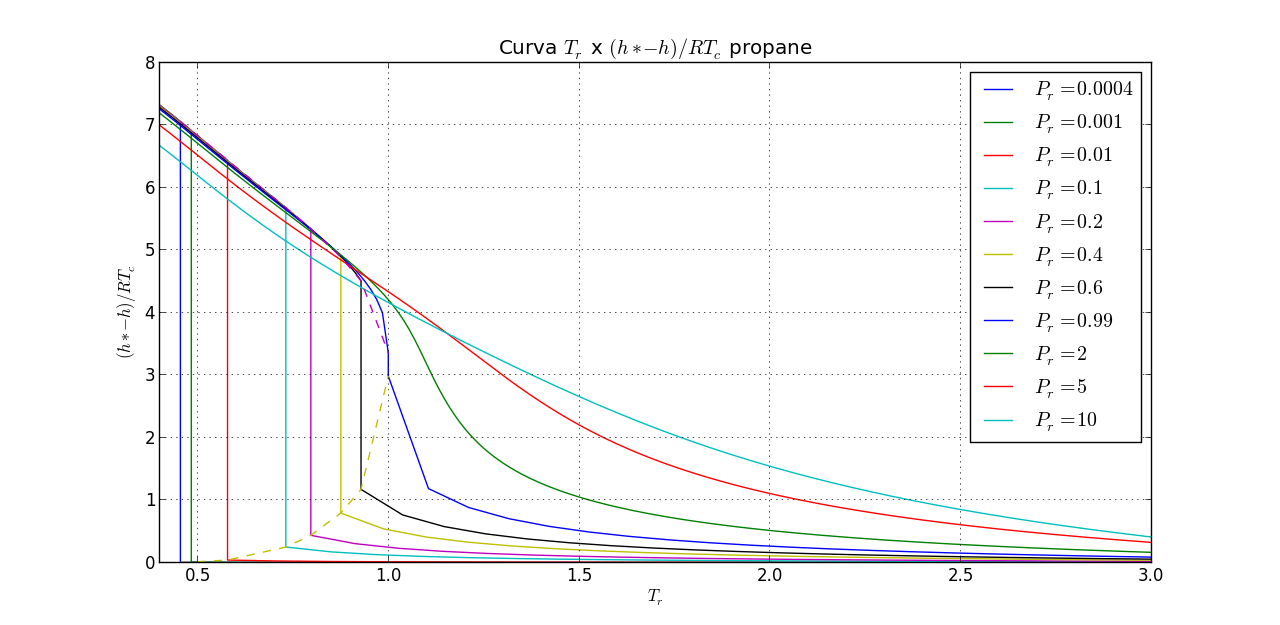
\includegraphics[%
            width=\textwidth
        ]   {propaneResidualEnthalpyPerTemperature.png}

        \label{fig:6.2}
    \end{figure}

    \begin{figure}[!htb]
        \caption{%
            Entalpia residual adimensional
            $\frac{\protect\idealgasprop{intEnthalpy} -
            \gls{intEnthalpy}}{\gls{gasConstant}\gsub{temperature}{critical}}$
            em função da pressão reduzida \gsub{pressure}{reduced} com a
            temperatura reduzida \gsub{temperature}{reduced}  como parâmetro.
        }
        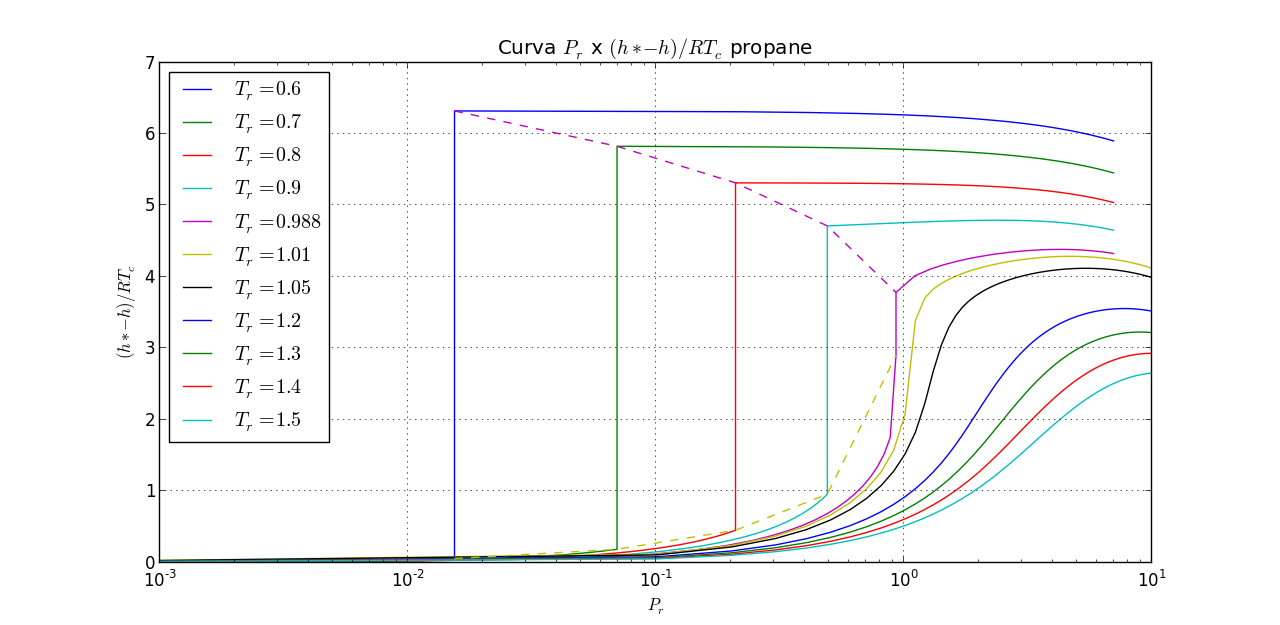
\includegraphics[%
            width=\textwidth
        ]   {propaneResidualEnthalpyPerPressure.png}

        \label{fig:6.3}
    \end{figure}


    \begin{figure}[!htb]
        \caption{%
            Entropia residual adimensional
            $\frac{\protect\idealgasprop{intEntropy} -
            \gls{intEntropy}}{\gls{gasConstant}}$ em função da temperatura
            reduzida \gsub{temperature}{reduced} com a pressão reduzida
            \gsub{pressure}{reduced}  como parâmetro.
        }
        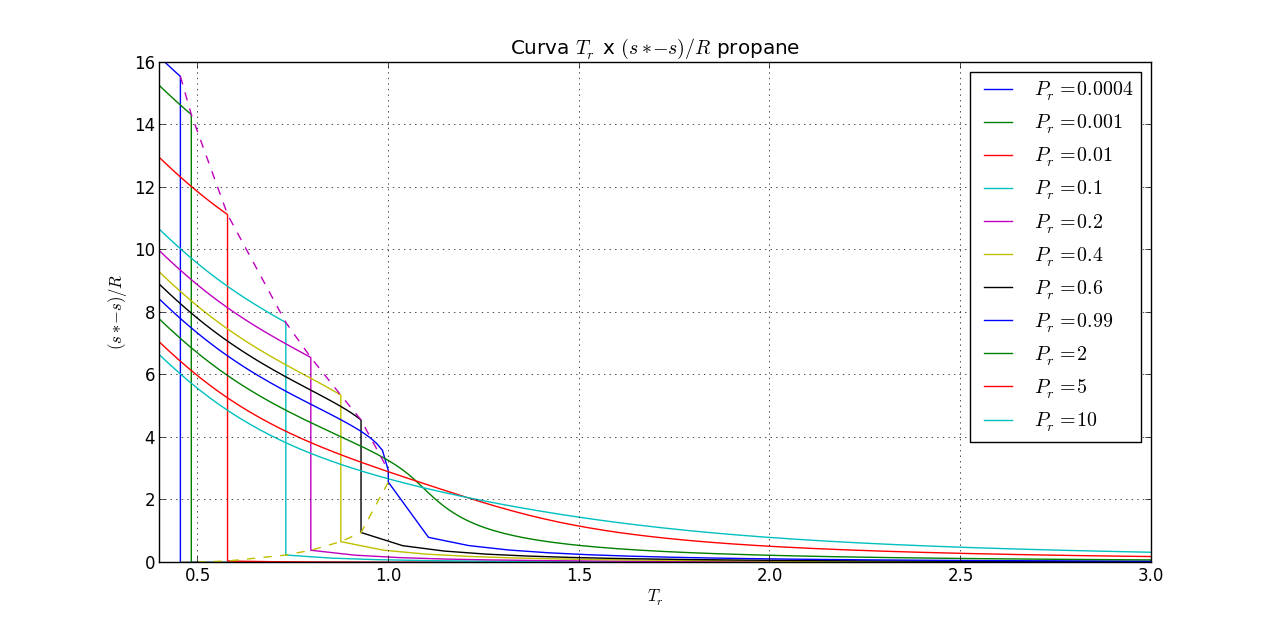
\includegraphics[%
            width=\textwidth
        ]   {propaneResidualEntropyPerTemperature.png}

        \label{fig:6.4}
    \end{figure}

    \begin{figure}[!htb]
        \caption{%
            Entropia residual adimensional
            $\frac{\protect\idealgasprop{intEntropy} -
            \gls{intEntropy}}{\gls{gasConstant}}$ em função da pressão reduzida
            \gsub{pressure}{reduced} com a temperatura reduzida
            \gsub{temperature}{reduced}  como parâmetro.
        }
        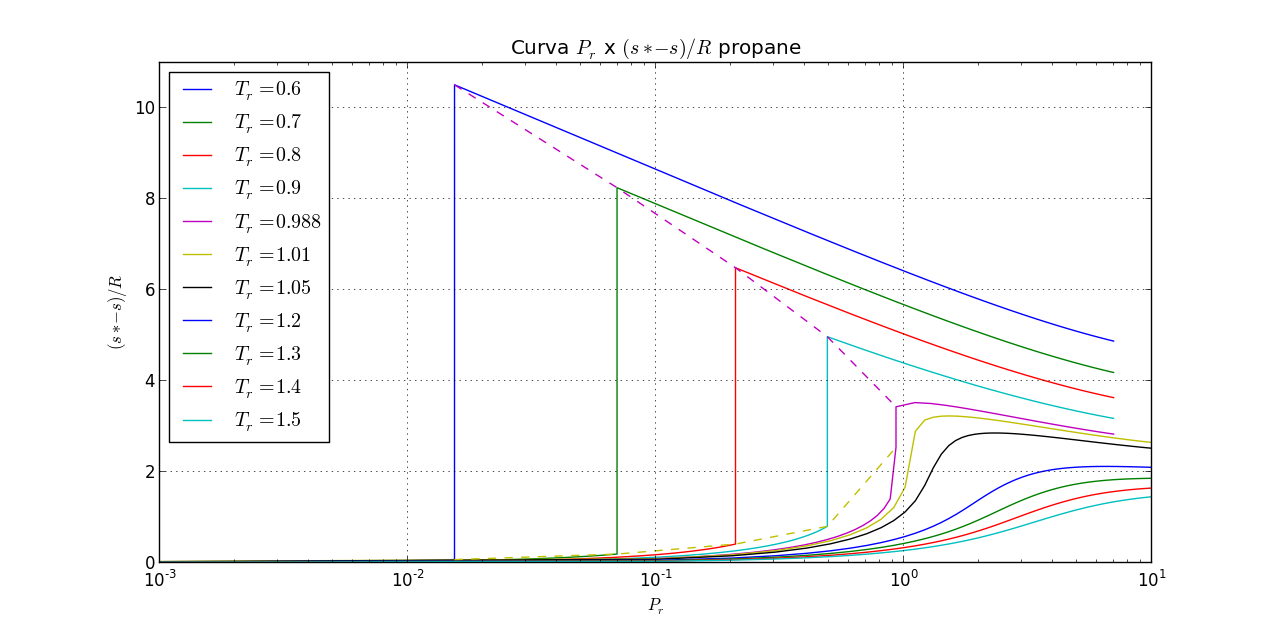
\includegraphics[%
            width=\textwidth
        ]   {propaneResidualEntropyPerPressure.png}

        \label{fig:6.5}
    \end{figure}

    \begin{figure}[!htb]
        \caption{%
            Coeficiente de fugacidade $\frac{\gls{fugacity}}{\gls{pressure}}$
            em função da temperatura reduzida \gsub{temperature}{reduced} com a
            pressão reduzida \gsub{pressure}{reduced}  como parâmetro.
        }
        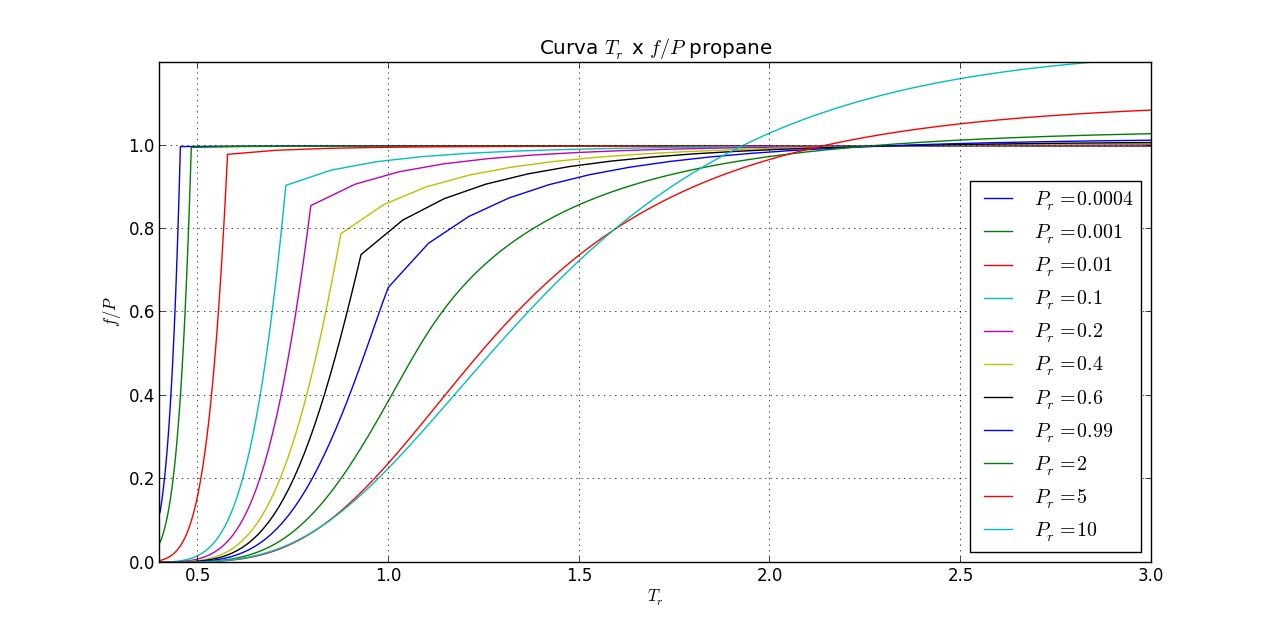
\includegraphics[%
            width=\textwidth
        ]   {propaneFugacityCoeffPerTemperature.png}

        \label{fig:6.6}
    \end{figure}

    \begin{figure}[!htb]
        \caption{%
            Coeficiente de fugacidade $\frac{\gls{fugacity}}{\gls{pressure}}$
            em função da pressão reduzida \gsub{pressure}{reduced} com a
            temperatura reduzida \gsub{temperature}{reduced} como parâmetro.
        }
        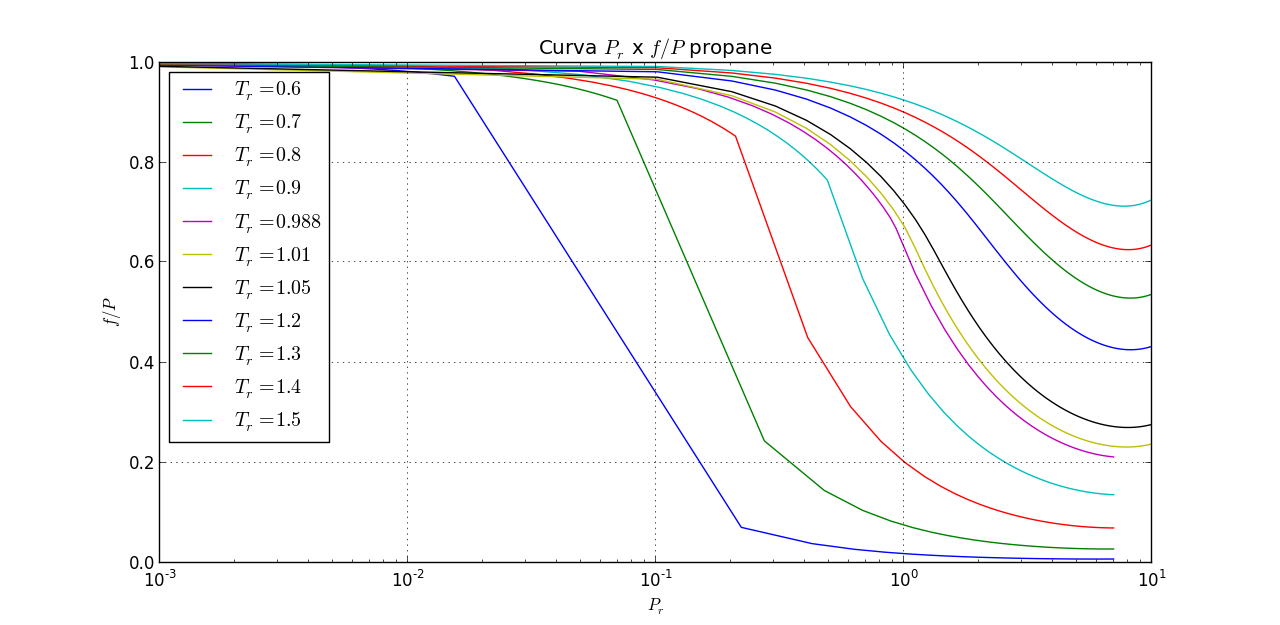
\includegraphics[%
            width=\textwidth
        ]   {propaneFugacityCoeffPerPressure.png}

        \label{fig:6.7}
    \end{figure}


    \newpage
    \section{Os Parâmetros de Expansividade e de Compressibilidade}

    Vamos definir mais algumas propriedades termodinâmicas úteis. A
    expansividade volumétrica, \gls{volumeExpansivity}, a compressibilidade
    isotérmica \gls{isothermalCompressibility} e a compressibilidade adiabática
    \gls{adiabaticCompressibility} serão dadas, respectivamente por:
    %
    \begin{equation}
    \label{eq:6.29}
        \gls{volumeExpansivity}
        \equiv
        \frac{1}{\gls{specificVolume}}
        \ddxconsty{
            \gls{specificVolume}
        }{
            \gls{temperature}
        }{
            \gls{pressure}
        }
        \functionOf{
            \gls{temperature},
            \gls{pressure}
        }\,,
    \end{equation}
    %
    que pode ser positiva ou negativa,
    %
    \begin{equation} \label{eq:6.30}
        \gls{isothermalCompressibility}
        \equiv
        -\frac{1}{\gls{specificVolume}}
        \ddxconsty{
            \gls{specificVolume}
        }{
            \gls{pressure}
        }{
            \gls{temperature}
        }
        \functionOf{
            \gls{temperature},
            \gls{pressure}
        }\,,
    \end{equation}
    %
    sempre positiva
    %
    \begin{equation} \label{eq:6.31}
        \gls{adiabaticCompressibility}
        \equiv
        -\frac{1}{\gls{specificVolume}}
        \ddxconsty{
            \gls{specificVolume}
        }{
            \gls{pressure}
        }{
            \gls{entropy}
        }\,
    \end{equation}
    %
    também sempre positiva.

    Você deve ter percebido que \gls{volumeExpansivity} e
    \gls{isothermalCompressibility} correspondem às derivadas parciais das
    equações de estado explícitas em \gls{specificVolume}. Estas propriedades
    podem ser obtidas experimentalmente. Levando-se em conta a Regra da
    Inversão, a única derivada parcial que ainda não foi definida é
    \ddxconsty{\gls{pressure}}{\gls{temperature}}{\gls{specificVolume}}. Pela
    Regra Cíclica, podemos escrever:
    %
    \begin{equation} \label{eq:6.32}
        \ddxconsty{
            \gls{pressure}
        }{
            \gls{temperature}
        }{
            \gls{specificVolume}
        }
        \ddxconsty{
            \gls{temperature}
        }{
            \gls{specificVolume}
        }{
            \gls{pressure}
        }
        \ddxconsty{
            \gls{specificVolume}
        }{
            \gls{pressure}
        }{
            \gls{temperature}
        }
        =
        -1\,,
    \end{equation}
    %
    ou
    %
    \begin{equation} \label{eq:6.33}
        \ddxconsty{
            \gls{pressure}
        }{
            \gls{temperature}
        }{
            \gls{specificVolume}
        }
        =
        -\dfrac{
            \ddxconsty{
                \gls{specificVolume}
            }{
                \gls{temperature}
            }{
                \gls{pressure}
            }
        }{
            \ddxconsty{
                \gls{specificVolume}
            }{
                \gls{pressure}
            }{
                \gls{temperature}
            }
        }
        =
        \frac{
            \gls{volumeExpansivity}
        }{
            \gls{isothermalCompressibility}
        }\,.
    \end{equation}

    Como podemos obter \gls{adiabaticCompressibility}? Lembre-se que:
    %
    \begin{equation}
        \gls{constPressureSpecificHeat}
        \functionOf{
            \gls{temperature},
            \gls{pressure}
        }
        =
        \ddxconsty{
            \gls{intEnthalpy}
        }{
            \gls{temperature}
        }{
            \gls{pressure}
        }
        =
        \gls{temperature}
        \ddxconsty{
            \gls{intEntropy}
        }{
            \gls{temperature}
        }{
            \gls{pressure}
        }\,,
    \end{equation}
    %
    e
    %
    \begin{equation}
        \gls{constVolumeSpecificHeat}
        \functionOf{
            \gls{temperature},
            \gls{specificVolume}
        }
        =
        \ddxconsty{
            \gls{intInternalEnergy}
        }{
            \gls{temperature}
        }{
            \gls{specificVolume}
        }
        =
        \gls{temperature}
        \ddxconsty{
            \gls{intEntropy}
        }{
            \gls{temperature}
        }{
            \gls{specificVolume}
        }\,.
    \end{equation}

    Utilizando a Regra Cíclica e a Regra da Quarta Propriedade na
    \cref{eq:6.31}, temos:
    %
    \begin{equation} \label{eq:6.34}
        \gls{adiabaticCompressibility}
        \equiv
        -\frac{1}{\gls{specificVolume}}
        \ddxconsty{
            \gls{specificVolume}
        }{
            \gls{pressure}
        }{
            \gls{intEntropy}
        }
        =
        \frac{1}{\gls{specificVolume}}
        \dfrac{
            \ddxconsty{
                \gls{intEntropy}
            }{
                \gls{pressure}
            }{
                \gls{specificVolume}
            }
        }{
            \ddxconsty{
                \gls{intEntropy}
            }{
                \gls{specificVolume}
            }{
                \gls{pressure}
            }
        }
        =
        \frac{
            \displaystyle
            \ddxconsty{
                \gls{intEntropy}
            }{
                \gls{temperature}
            }{
                \gls{specificVolume}
            }
            \ddxconsty{
                \gls{temperature}
            }{
                \gls{pressure}
            }{
                \gls{specificVolume}
            }
        }{
            \displaystyle
            \ddxconsty{
                \gls{intEntropy}
            }{
                \gls{temperature}
            }{
                \gls{pressure}
            }
            \ddxconsty{
                \gls{temperature}
            }{
                \gls{specificVolume}
            }{
                \gls{pressure}
            }
        }
        =
        \frac{1}{\gls{specificVolume}}
        \frac{
            \gls{constVolumeSpecificHeat}
            \frac{
                \gls{isothermalCompressibility}
            }{
                \gls{volumeExpansivity}
            }
        }{
            \dfrac{
                \gls{constPressureSpecificHeat}
            }{
                \gls{volumeExpansivity}
                \gls{specificVolume}
            }
        }
        =
        \left(
            \frac{
                \gls{constVolumeSpecificHeat}
            }{
                \gls{constPressureSpecificHeat}
            }
        \right)
        \gls{isothermalCompressibility}\,.
    \end{equation}

    Qual a relação entre \gls{constPressureSpecificHeat} e
    \gls{constVolumeSpecificHeat}? Vejamos. Igualando as \cref{eq:5.40,eq:5.45}
    expandindo \diff{\gls{specificVolume}} como função de
    \gls{pressure},\gls{temperature}:
    %
    \begin{equation} \label{eq:6.35}
        \left[
            \frac{
                \gls{constPressureSpecificHeat}
                -
                \gls{constVolumeSpecificHeat}
            }{
                \gls{temperature}
            }
            -
            \ddxconsty{
                \gls{pressure}
            }{
                \gls{temperature}
            }{
                \gls{specificVolume}
            }
            \ddxconsty{
                \gls{specificVolume}
            }{
                \gls{temperature}
            }{
                \gls{pressure}
            }
        \right]
        \diff{\gls{temperature}}
        +
        \left[
            \ddxconsty{
                \gls{pressure}
            }{
                \gls{temperature}
            }{
                \gls{specificVolume}
            }
            \ddxconsty{
                \gls{specificVolume}
            }{
                \gls{pressure}
            }{
                \gls{temperature}
            }
            \ddxconsty{
                \gls{specificVolume}
            }{
                \gls{temperature}
            }{
                \gls{pressure}
            }
        \right]
        \diff{\gls{pressure}}
        =
        0\,.
    \end{equation}

    Ambos os coeficientes tem que ser nulos. O segundo coeficiente é novamente
    a Regra Cíclica. Substituindo-se pelos valores de \gls{volumeExpansivity}
    e \gls{isothermalCompressibility} no primeiro coeficiente, obtemos:
    %
    \begin{equation} \label{eq:6.36}
        \gls{constPressureSpecificHeat}
        -
        \gls{constVolumeSpecificHeat}
        =
        \frac{
            \gls{temperature}
            \gls{specificVolume}
            \gls{volumeExpansivity}^2
        }{
            \gls{isothermalCompressibility}
        }\,.
    \end{equation}

    Aplicando a Regra da Cadeia, a Regra da Inversão, a Regra das Derivadas
    Cruzadas e a Regra da Quarta Propriedade, bem como as Relações de Maxwell e
    as Relações Fundamentais, você pode demonstrar uma infinidade de
    identidades termodinâmicas e associá-las à determinação da propriedades
    termodinâmicas a quatro parâmetros.

    \section{Próximos Passos}

    Finalmente, reafirmamos que:

    \begin{enumerate}
        \item Todos os problemas de Termodinâmica que não tenham misturas
            reativas podem ser expressos na forma de diferenças de propriedades
            termodinâmicas intensivas entre todos os estados;

        \item Qualquer massa ou vazão de massa (ou número de moles ou vazão
            molar) sempre pode ser utilizada como fator de escala em qualquer
            problema;

        \item O estado termodinâmico intensivo dimensional de qualquer
            substância pura está completamente definido pelas --- por nós
            denominadas --- propriedades primárias, que são
            $(\gls{pressure},\gls{temperature})$, quando independentes, ou
            então $(\gls{pressure},\gls{vaporQuality})$ ou
            $(\gls{temperature},\gls{vaporQuality})$ na saturação;

        \item Todos os problemas em Termodinâmica podem ser adimensionalizados.
            Os estados adimensionais a quatro parâmetros dependem de
            $\gsub{temperature}{reduced}, \gsub{pressure}{reduced},
            \gls{PitzerAcentricFactor}, \gls{WuPolarFactor}$ e não dependem de
            nenhuma base arbitrária;

        \item A assinatura de qualquer substância pura é dada por
            $(\gls{molecularMass}, \gsub{temperature}{critical},
            \gsub{pressure}{critical}, \gls{PitzerAcentricFactor},
            \gls{WuPolarFactor})$. Para resolver problemas, precisamos conhecer
            também o comportamento de
            $\idealgasprop{constPressureSpecificHeat}\functionOf{\gls{temperature}}$,
            que é o calor específico a pressão constante do gás perfeito da
            substância pura.
    \end{enumerate}

    Parabéns, agora você tem o domínio completo, no que se refere a substâncias
    puras, as aplicações da Primeira e Segunda Leis da Termodinâmica e
    combinação, a produção de identidades termodinâmicas e a determinação de
    propriedades mensuráveis e não mensuráveis, com o apoio de
    \command{LK\_proptermo} e a equação de estado a quatro parâmetros de
    Lee-Kesler-Wu-Stiel.

    Nos próximos capítulos aprenderemos a lidar com misturas homogêneas e não
    homogêneas, não reativas e reativas, em equilíbrio químico e de fases. TUDO
    o que você aprendeu até aqui é muito importante e TUDO será utilizado como
    fundamento para os nossos próximos avanços.
